\documentclass[11pt]{article}
\usepackage[utf8]{inputenc}
\usepackage[T1]{fontenc}
\usepackage{lmodern}
\usepackage[margin=1in]{geometry}
\usepackage{amsmath,amssymb}
\usepackage{booktabs}
\usepackage{adjustbox}
\usepackage{graphicx}
\usepackage{microtype}
\usepackage{url}
\usepackage[hidelinks]{hyperref}
\usepackage[font=small]{caption}
\graphicspath{{figures/}{./}}  % figures may sit in figures/ or beside main.tex (e.g. on Overleaf)

\title{When Should a Finance AI Stay Silent? Selective Answering for Financial-Filings QA, Measured Honestly}
\author{Mohammed Arshan O \\ Independent researcher \\ \texttt{arshan.ottakath@gmail.com}}
\date{November 2026}

\begin{document}
\maketitle



\begin{abstract}

Large language models answer questions about SEC filings well enough to be tempting and badly enough to be dangerous --- so the deployment question is not ``how accurate is the model?'' but ``when should it be allowed to answer at all?'' We measure selective answering end-to-end on expert-written filings QA with three tiers of one frontier model family (Claude Haiku 4.5, Sonnet 5, Opus 5) on FinanceBench (150 questions; oracle-evidence and closed-book settings) and a seeded 40-item FailSafeQA subset, comparing three practical confidence signals --- (M1) verbalized 0--100 confidence, (M2) paraphrase self-agreement, (M3) a judge-free evidence-presence check --- under a pre-registered, frozen-output protocol with held-out threshold calibration. Four findings. \textbf{(1)} With gold evidence and an explicit ``CANNOT ANSWER'' option, error among answered questions is already 7.7--10.1\% \emph{before any thresholding}: at a 10\% risk target, tuned confidence thresholds turn out to bind almost nothing --- the models' own refusals do the work --- and whether the target is met on a held-out half depends on the split (met in 49--88\% of 200 random splits). \textbf{(2)} Decontaminated self-agreement is the most \emph{reliable} rule we test: for the small tier it meets the 10\% target in 98.5\% of splits at $\sim$84\% coverage. \textbf{(3)} Nothing is certifiable: a rule that demands a finite-sample statistical bound (exact binomial, 95\%) before answering certifies zero coverage at either 5\% or 10\% with a 75-question calibration set --- a concrete measurement of how much calibration data risk-\emph{guaranteed} filings QA actually needs. \textbf{(4)} On perturbed FailSafeQA items with the abstention option present, fabrication on unanswerable inputs was 0/118 pooled (exact 95\% upper bound 2.5\%) while 82.5--90\% of perturbed-answerable items were still answered correctly --- a striking contrast, though not a causal one, with the 41\% fabrication the FailSafeQA authors report for the most robust model under their protocol. All raw outputs were frozen before analysis; the design, every mid-course deviation, and this revision are logged in a version-controlled rulebook.

\end{abstract}

\section{Introduction}

Financial-filings QA has a measured honesty problem. FinanceBench found GPT-4-Turbo with retrieval incorrectly answered or refused 81\% of questions (Islam et al., 2023); FailSafeQA reports its most robust frontier model fabricating answers on 41\% of perturbed or context-degraded inputs while the most compliant over-refuses (Kamble et al., 2025); FinTrust (2025) reports overconfidence on unanswerable financial questions. Regulated deployment needs an \emph{operating rule}: answer only when a confidence signal clears a threshold chosen to keep the error rate among answers below a target.

Selective prediction supplies the machinery. To our knowledge --- from a 107-paper limitations review (\S{}2), re-verified by fresh sweeps in August and November 2026 --- no published study applies risk-targeted selective answering to financial-filings QA benchmarks. The nearest neighbours either hold an error target on \emph{other} financial tasks --- conformal risk control for VLM-extracted invoice and form fields (Jin et al., 2026) and error-budget operating points for financial chart and document-image VQA (Khanmohammadi et al., 2026) --- or answer selectively on filings and annual-report QA \emph{without} an error target: VeriFin (2026) accepts only numeric answers it can verify against XBRL facts, and CLAIR-Fin (2026) abstains by a fixed audit rule. General-domain risk-controlled selective QA (COIN, 2026; CIC, 2026; A-CRC-QA, 2026) and conformal abstention for financial \emph{forecasting} (FinAbstain, 2026) complete the neighbourhood. We supply the missing measurement, deliberately isolated from retrieval: models receive the gold evidence pages, so every failure is a failure of \emph{knowing when not to answer}.

Contributions: \textbf{(1)} the first pre-specified, frozen-output measurement of what \emph{risk-targeted} selective answering buys on expert-written filings QA, across three capability tiers and three deployable signals, with the operating points a compliance team would actually use; \textbf{(2)} an honest account of the statistics: plug-in thresholds vs. certified (exact-bound) thresholds, split-sensitivity over 200 seeds, and the negative result that finite-sample certification is impossible at n$\approx$75 calibration questions; \textbf{(3)} evidence that with an explicit abstention affordance, fabrication on unanswerable perturbed inputs is at most 2.5\% pooled (95\% upper bound) at our scale, alongside a candid list of confounds that prevent a causal comparison with prior benchmark reports; \textbf{(4)} a fully reproducible artifact: pre-registered rulebook with a complete deviation log (including an adversarial internal review that reshaped this draft), frozen raw outputs, and a no-API-key Run-All notebook.


\section{Related work}

\textbf{Benchmarks that measure the failure.} FinanceBench (Islam et al., 2023): 150 expert questions over SEC filings with gold evidence; documented the refusal-vs-hallucination trade-off. FailSafeQA (Kamble et al., 2025): query and context perturbations over long filings, scoring robustness against compliance with an LLM judge. FinTrust (2025); FinVerBench (2026): calibration-adjacent findings on financial tasks. Our 107-paper review tags hallucination/abstention as a stated limitation in $\sim$20 papers; FinRAG-12B (2026) fine-tunes for refusals in retail banking without risk targets.

\textbf{Closest work since mid-2026.} Error targets have reached adjacent financial tasks. Jin et al. (2026) apply conformal risk control at a $<$10\% error target to key-value fields that VLMs extract from invoices and forms, and find that the models' verbalized confidence clears only 0.1--7.0\% of fields under that target. Khanmohammadi et al. (2026) report error-budget ``safe yield'' for financial chart and document-image VQA --- near zero at a 5\% budget when pooled across models --- with thresholds fitted on the evaluation data and a rephrasing-ensemble signal related to our M2. On filings QA itself, selective answering exists without an error target: VeriFin (2026) verifies numeric answers against XBRL facts with an SMT solver and abstains otherwise, reporting 100\% observed precision among accepted answers on sets that include 67 FinanceBench questions; CLAIR-Fin (2026) abstains by a fixed claim-audit rule on central-bank annual-report QA; FinSAgent (2026) handles insufficient evidence by prompt instruction only. None of these chooses an answering threshold to meet a stated error target on filings QA and tests it on held-out questions --- the measurement we supply.

\textbf{Selective prediction and risk control.} Verbalized confidence (Lin et al., 2022; Tian et al., 2023), self-consistency (Wang et al., 2023), risk--coverage analysis (Geifman \& El-Yaniv, 2017), conformal risk control (Angelopoulos et al., 2022), and provable selective QA (COIN, 2026; A-CRC-QA, 2026) are established outside finance. Our certified rule (\S{}3.5) is the Clopper--Pearson threshold calibration used for selective QA by COIN (2026) and CIC (2026); UniCR (2025) enforces an error budget by conformal refusal over fused uncertainty signals. Kotte (2026) analyses when conformal risk control can and cannot certify LLM outputs --- including a minimum abstention fraction whenever base risk exceeds the target --- and compares finite-sample bounds; our certification failure (\S{}4.4c) is a filings-QA measurement of those limits at n$\approx$75, not a new phenomenon. We do not extend this methodology; we measure what it delivers on filings QA, including where its guarantees are vacuous at realistic calibration sizes.


\section{Method}


\subsection{Data}
\begin{itemize}
\item \textbf{FinanceBench open set}: 150 questions (50 metrics-generated / 50 domain-relevant / 50 novel-generated; 32 companies; up to 7 questions share a filing --- a clustering limitation, \S{}6). \emph{Oracle-evidence}: gold evidence pages provided. \emph{Closed-book}: no document.
\item \textbf{FailSafeQA}: seeded subset of 40/220 items (seed 20260807; quota-forced scope cut, logged before any run). Per item, 3 conditions: \textbf{base} (clean query + full filing, $\sim$32k tokens); one \textbf{perturbed-answerable} rotated over \{misspelled, incomplete, out-of-domain rephrase, OCR-corrupted context\}; one \textbf{unanswerable} rotated over \{context removed, out-of-scope query\}.
\end{itemize}



\subsection{Models and protocol}
Claude Haiku 4.5 / Sonnet 5 / Opus 5, accessed through the Claude Code agent harness (subscription path; the pre-registered API path was unaffordable), reasoning effort pinned to ``medium''. One item-level ask protocol throughout: answer only from the provided document; reply exactly ``CANNOT ANSWER'' if it lacks the information; output \path{ANSWER:} + \texttt{CONFIDENCE: \textless{}0\textendash{}100\textgreater{}}. Items were delivered under two packing regimes: one-per-sitting (605 sittings) and multi-item exam papers (FinanceBench papers: mean 9.8 items, max 12; FailSafeQA papers: mean 2.3, max 3) with an explicit item-independence header --- adopted mid-run when per-question harness overhead consumed $>$95\% of tokens; both the switch and its risks are logged (rulebook v1.3/v1.5) and probed in \S{}4.6. The harness wrapper means the measured system is ``model + fixed thin agent scaffold'', not a bare API call (\S{}6).


\subsection{Confidence signals}
\begin{itemize}
\item \textbf{M1 --- verbalized confidence}: the stated integer. Defined on all questions.
\item \textbf{M2 --- paraphrase self-agreement}: each question paraphrased once (pinned prompt, frozen pre-run); signal = the two answers agree (numeric within 1\%; text via pinned same-answer judge); refusal on either side = disagree. \textbf{Scope correction (v1.8):} 117/450 pairs had both askings inside one exam paper, breaking independence; they are excluded. Valid pairs: 112 (Haiku), 112 (Sonnet), 109 (Opus); M2 metrics use this eligible population.
\item \textbf{M3 --- evidence-presence check}: judge-free string check --- does the answer's number appear in the evidence after normalising commas, currency, parenthesised negatives, percents, $\times$10$^{3}$/$\times$10$^{6}$ re-expressions? Per pre-registration, defined only on numeric-gold oracle questions (n=53 per tier; an earlier all-questions computation was a scope bug, corrected in v1.8).
\end{itemize}



\subsection{Grading}
Numeric-gold questions (433 rows): deterministic parser --- 1\% relative tolerance in the question's stated unit, plus half a unit in the gold's last printed decimal; clean power-of-ten mismatches flagged as scale errors and graded wrong. Text-gold questions (966 rows): pinned AI grader (mid tier). Refusals (191) and unanswerable-condition rows (118) detected deterministically. The 61 parser-incorrect rows also received a grader second opinion; 4 disagreed. Audit: the large tier re-graded 63 grades (60 seeded random --- of which one coincided with a disagreement row --- plus the remaining flagged rows): overall agreement 59/63 (93.7\%, Cohen's $\kappa$ 0.78); random-sample agreement 59/60. All 4 disagreements were resolved against the parser by both AI graders and adjudicated to the majority verdict; because this second-opinion pipeline only re-examines parser-\emph{incorrect} rows it can only raise accuracy, so \S{}4.4 reports pre- and post-adjudication results side by side. A 10-question pilot was hand-audited in full before the main runs (one grader fix, logged). The author then hand-graded a simple random sample of 30 of the 1,708 grades (seed 30303; \path{src/make_human_audit.py}; \path{results/audit_sheet_human.csv}) using a helper that hides the pipeline grade until a verdict is entered (it does not log later changes), and agreed with the pipeline on 29/30 (96.7\%, exact 95\% CI [82.8, 99.9]; Cohen's $\kappa$ 0.92). Six sampled rows were deterministic refusal or compliance grades; on the other 24, agreement was 23/24 (95.8\%, CI [78.9, 99.9]). The single disagreement was a text-gold judgement question (3M, FY2022: is the business capital-intensive?), where the AI grader accepted ``moderately capital-intensive'' against a gold answer of ``No'' and the author graded it incorrect --- a lenient AI-grader call that, like the one-directional adjudication above, would bias accuracy upward if systematic. One isolated disagreement does not meet the rulebook's ``systematically wrong'' trigger for a fix and full re-grade, so grades were not changed.


\subsection{Operating rules (plug-in and certified)}
Graded oracle answers are split 50/50 by question (primary seed 20260807) into tuning and proving halves. \textbf{Plug-in rule (pre-registered):} smallest threshold \emph{t} whose tuning-half empirical selective risk $\leq$ target. \textbf{Certified rule (added in v1.8):} smallest \emph{t} whose one-sided 95\% exact (Clopper-Pearson) upper bound on tuning-half risk $\leq$ target --- the finite-sample-safe analogue. Chosen rules are applied untouched to the proving half; we report coverage, n answered, realized risk, and exact 95\% intervals; rows with n$<$20 answered are flagged degenerate. Split-sensitivity: the entire procedure re-run over 200 random splits. We do not use the word \emph{guarantee} for the plug-in rule.


\section{Results}

n=150 questions per tier per setting (FinanceBench); FailSafeQA sittings 118 (Haiku; both lost sittings were out-of-scope items) / 120 / 120. Accuracies carry exact 95\% CIs in brackets.


\subsection{Accuracy, refusal, and the closed-book gap}

\begin{center}\small
\begin{adjustbox}{max width=\linewidth}
\begin{tabular}{lccc}
\toprule
 & Haiku 4.5 & Sonnet 5 & Opus 5 \\
\midrule
Oracle accuracy (all 150) & 82.7\% [75.6, 88.4] & 88.0\% [81.7, 92.7] & 91.3\% [85.6, 95.3] \\
Oracle accuracy (among answered) & 89.9\% & 92.3\% & 91.9\% \\
Oracle refusal rate & 8.0\% & 4.7\% & 0.7\% \\
Closed-book accuracy & 18.7\% [12.8, 25.8] & 44.7\% [36.6, 53.0] & 68.7\% [60.6, 76.0] \\
Closed-book refusal rate & 54.0\% & 28.0\% & 10.0\% \\
\bottomrule
\end{tabular}
\end{adjustbox}
\end{center}


Accuracy rises with tier and refusal falls, but the Sonnet--Opus accuracy gap is within paired noise at n=150, and the \emph{signal-quality} ordering is not monotonic (\S{}4.2--4.3) --- we therefore do not claim a clean capability ladder. Scale errors (the classic $\times$1000 slip): none in the whole study. The parser's scale flag fired twice and both flags are false positives on inspection: a scale word from a neighbouring number attached to a correct ``4.2\%'' (Opus, paraphrase; adjudicated correct), and a unit-correct ``9,200 million'' against a gold of 9,068 whose absolute value lies within the flag's 2\% tolerance of 10$^{6}\times$ the gold (Haiku, closed-book; still graded wrong, on value). The closed-book results show substantial memorised knowledge of these filings (up to 68.7\%), which inflates confidence--correctness alignment in unquantified ways: all oracle-setting numbers should be read as \emph{for questions partially familiar from pretraining} (\S{}6).


\subsection{What each signal offers (full-sample operating points)}

On eligible populations: M1 (all 150), M2 (valid pairs 112/112/109), M3 (numeric-gold, 53).

\begin{center}\small
\begin{adjustbox}{max width=\linewidth}
\begin{tabular}{lccc}
\toprule
Signal & Haiku & Sonnet & Opus \\
\midrule
M1: matched-coverage mean risk (cov 0.2--0.9) & 4.7\% & 4.6\% & 3.3\% \\
M1: in-sample coverage at $\leq$10\% risk & 90.0\% & 95.3\% & 99.3\% \\
M1: in-sample coverage at $\leq$5\% risk & 78.0\% & 80.7\% & 86.7\% \\
M2: coverage / risk & 83.9\% / 5.3\% & 82.1\% / 7.6\% & 93.6\% / 8.8\% \\
M3: coverage / risk & 83.0\% / 11.4\% & 81.1\% / 7.0\% & 81.1\% / 7.0\% \\
\bottomrule
\end{tabular}
\end{adjustbox}
\end{center}


In-sample coverages are maximally-selected statistics and overstate what a deployed rule achieves --- \S{}4.4 gives the held-out picture. M3, restricted to its defined scope, is the weakest and noisiest signal (n=53).

\begin{figure}[tb]
\centering
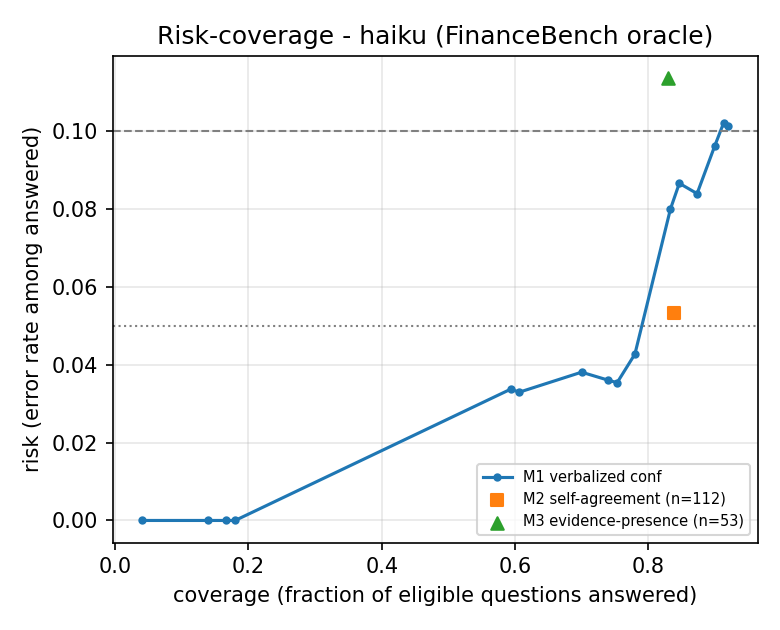
\includegraphics[width=0.32\linewidth]{risk_coverage_haiku.png}
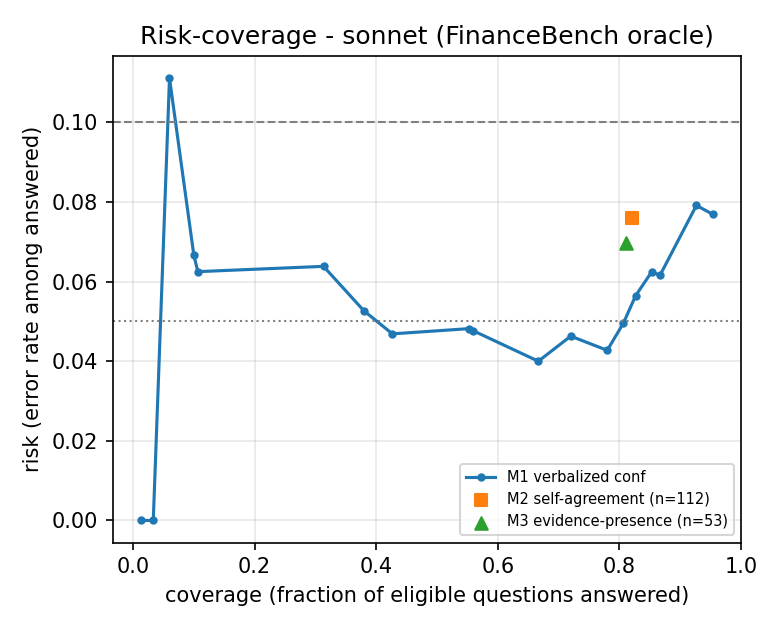
\includegraphics[width=0.32\linewidth]{risk_coverage_sonnet.png}
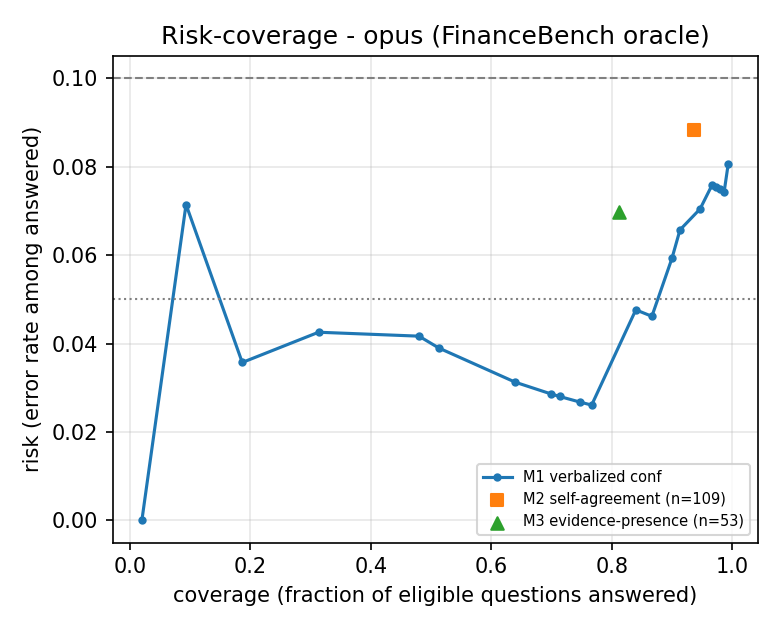
\includegraphics[width=0.32\linewidth]{risk_coverage_opus.png}
\caption{Risk--coverage on FinanceBench with gold evidence (left to right: Haiku 4.5, Sonnet 5, Opus 5). The line sweeps the M1 verbalized-confidence threshold; the square and triangle are the single operating points of M2 (paraphrase self-agreement, valid pairs only) and M3 (evidence-presence check, numeric-gold questions only). Dashed and dotted lines mark the 10\% and 5\% risk targets. Full-sample curves; held-out operating points are in \S4.4.}
\label{fig:rc}
\end{figure}


\subsection{Calibration}

Decile-bin ECE on answered questions: 4.6\% (Haiku, n=138), 9.4\% (Sonnet, n=143), 4.3\% (Opus, n=149). Reliability diagrams are near-diagonal in aggregate, but individual bins are small and noisy --- e.g. Haiku's [80,90) bin holds 16 answers at 56\% accuracy --- so we claim aggregate calibration only, note that ECE at n$\approx$150 is bin-sensitive, and observe that the \emph{mid} tier is the worst-calibrated of the three. Relative to the systematic overconfidence reported on earlier model generations, these are small errors; they are not bin-level reliability.

\begin{figure}[tb]
\centering
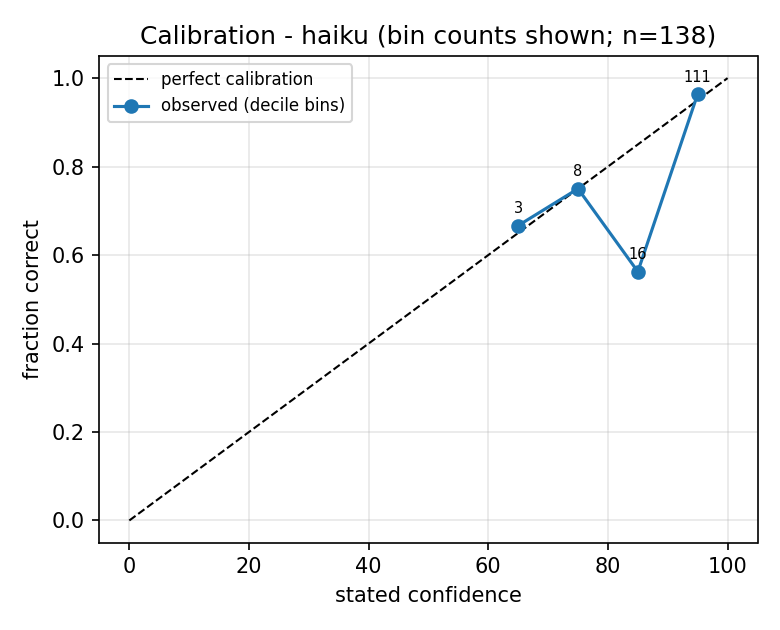
\includegraphics[width=0.32\linewidth]{calibration_haiku.png}
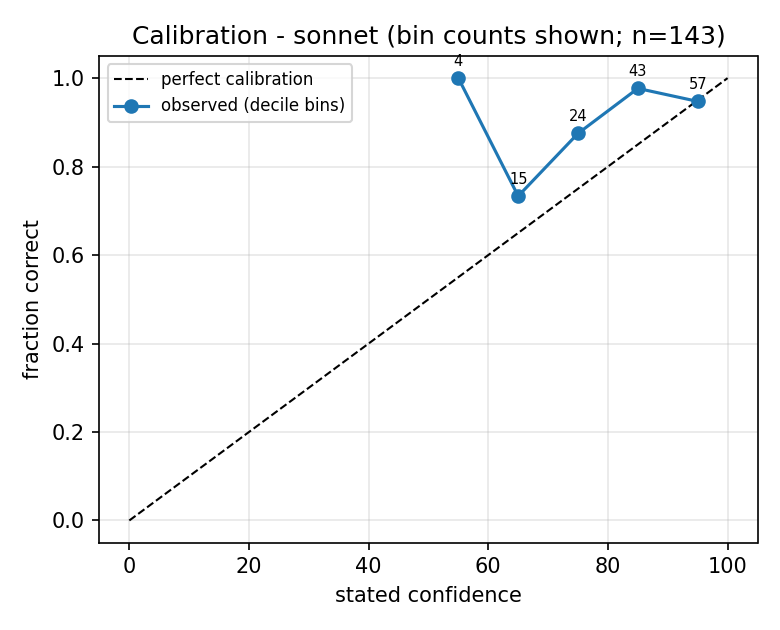
\includegraphics[width=0.32\linewidth]{calibration_sonnet.png}
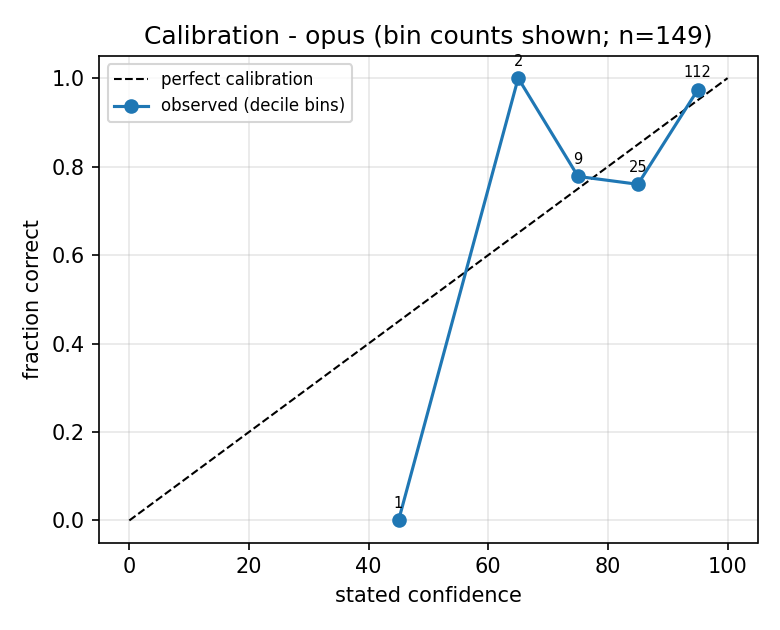
\includegraphics[width=0.32\linewidth]{calibration_opus.png}
\caption{Reliability of M1 verbalized confidence on answered gold-evidence questions (left to right: Haiku 4.5, $n=138$; Sonnet 5, $n=143$; Opus 5, $n=149$). Points are decile bins of stated confidence, annotated with bin counts; the dashed line is perfect calibration. Bins are small, so we claim aggregate calibration only (\S4.3).}
\label{fig:cal}
\end{figure}


\subsection{Held-out operating points, certification, and split-sensitivity}

Primary seed (20260807), plug-in rule:

\begin{center}\small
\begin{adjustbox}{max width=\linewidth}
\begin{tabular}{lcccccc}
\toprule
Model & Signal & Target & Coverage & n ans. & Realized risk [95\% CI] & Note \\
\midrule
Haiku & M1 & 10\% & 94.7\% & 71 & 11.3\% [5.0, 21.0] & threshold excluded 0 answers \\
Sonnet & M1 & 10\% & 98.7\% & 74 & 6.8\% [2.2, 15.1] & threshold excluded 0 answers \\
Opus & M1 & 10\% & 100.0\% & 75 & 8.0\% [3.0, 16.6] & threshold excluded 0 answers \\
Haiku & M2 & 10\% & 85.2\% & 46 & 2.2\% [0.1, 11.5] &  \\
Sonnet & M2 & 10\% & 90.7\% & 49 & 6.1\% [1.3, 16.9] &  \\
Opus & M2 & 10\% & 94.2\% & 49 & 8.2\% [2.3, 19.6] &  \\
Haiku & M1 & 5\% & 18.7\% & 14 & 0.0\% [0.0, 23.2] & degenerate (n$<$20) \\
Sonnet & M1 & 5\% & 4.0\% & 3 & 0.0\% [0.0, 70.8] & degenerate \\
Opus & M1 & 5\% & 2.7\% & 2 & 0.0\% [0.0, 84.2] & degenerate \\
\bottomrule
\end{tabular}
\end{adjustbox}
\end{center}


Three honest readings. \textbf{(a) At 10\%, the thresholds are inert.} For all three tiers the selected M1 threshold excludes zero additional answers on the proving half: coverage equals the non-refusal rate, and the achieved risk is the model's native error-among-answered. The models' built-in refusal behaviour already sits at the 10\% boundary; thresholding adds nothing there. \textbf{(b) At 5\%, plug-in thresholds certify nothing usable.} The surviving operating points answer 2--14 questions; their intervals extend to 23--84\%. \textbf{(c) The certified rule certifies nothing at all.} Requiring an exact 95\% upper bound $\leq$ target on the tuning half yields zero answerable coverage for every tier at both targets: with 75 calibration questions, certification needs at least 29 answered tuning items even with zero errors at the 10\% target, and at least 59 at 5\% --- and no threshold gets there. Risk-\emph{guaranteed} selective filings QA needs a calibration set several times larger than half of FinanceBench --- a concrete design requirement for future benchmarks, and the filings-QA face of the general certification limits analysed by Kotte (2026).

\textbf{Split-sensitivity (200 random splits, plug-in):} M1@10\% meets the target in 49\% (Haiku), 87.5\% (Sonnet), 86\% (Opus) of splits --- for the small tier it is a coin flip. M2@10\% meets it in 98.5\% (Haiku), 62.5\% (Sonnet), 37.5\% (Opus) of splits at median coverage 84/81/93\% --- making decontaminated self-agreement the most reliable 10\% rule for the small tier, while for the large tier simply \emph{answering everything it doesn't refuse} is as defensible as any rule tested. M1@5\% meets the target in only 43--64\% of splits. \textbf{Adjudication sensitivity:} under the pre-adjudication grades, the only headline row that changes is Sonnet M1@10\% (coverage 86.7\%, realized 4.6\% [1.0, 12.9]); Haiku and Opus rows are identical.


\subsection{FailSafeQA: guessing when you shouldn't}

\begin{center}\small
\begin{adjustbox}{max width=\linewidth}
\begin{tabular}{lccc}
\toprule
 & Haiku & Sonnet & Opus \\
\midrule
Base accuracy (n=40) & 85.0\% & 90.0\% & 95.0\% \\
Base refusal (over-refusal cost) & 2/40 & 2/40 & 0/40 \\
Robustness: perturbed-answerable acc. (n=40) & 82.5\% [67.2, --] & 87.5\% [73.2, --] & 90.0\% [76.3, --] \\
Compliance: refusal on unanswerable & 38/38 & 40/40 & 40/40 \\
Fabrication (95\% exact upper bound) & 0\% ($\leq$7.6\%) & 0\% ($\leq$7.2\%) & 0\% ($\leq$7.2\%) \\
\bottomrule
\end{tabular}
\end{adjustbox}
\end{center}


Pooled across tiers: \textbf{0/118 fabrications, exact 95\% upper bound 2.5\%.} Robustness costs 2.5--5 points versus clean baseline (differences within paired noise at n=40), and the small over-refusal cost (2/40 clean items refused by the smaller tiers) is the compliance side's price. Per-variant cells (n=8--12) are reported in \path{results/fsq_table.csv} as indicative only and we draw no per-variant conclusions. \textbf{Cross-study contrast, stated carefully:} the FailSafeQA authors report their most robust model fabricating on 41\% of perturbed/degraded inputs. Our 0/118 was obtained with different models, a different prompt that makes abstention an explicit legitimate output, a different (non-LLM-judge) scoring protocol, and a 40-item subset --- so we report the contrast as motivation for a controlled experiment, not as a causal finding. The pre-registered next step is a no-abstention-instruction control arm on the same items.


\subsection{Protocol equivalence and instrument validity}

Batching equivalence (pre-registered n=30; 26 pairs mapped, 4 attrition; mid tier, oracle only): refusal 1/26 vs 1/26; mean confidence 80.7 (batched) vs 82.8 (single); numeric-arm accuracy 9/10 vs 9/10; 9/10 numeric answers identical within 1\%. These are consistent with equivalence but underpowered to establish it; batching remains a disclosed threat (\S{}6). Grading validity rests on: deterministic parsing for all numeric golds, 93.7\% cross-tier audit agreement ($\kappa$ 0.78), the 10-question hand-audited pilot, and the author's 29/30 hand audit (\S{}3.4) --- with the caveat that both AI graders share the subjects' model family.


\section{Discussion}

What should a deployer take away? \textbf{First, the abstention affordance is doing most of the visible work.} With gold evidence and permission to refuse, these models' unthresholded error-among-answered already sits at 7.7--10.1\%, their refusals absorb the worst inputs, and on unanswerable perturbed inputs fabrication was undetected at our scale ($\leq$2.5\% pooled, 95\% bound). \textbf{Second, signal choice matters most below the native operating point.} Confidence thresholds bind only for targets stricter than $\sim$10\%; there, nothing we tested is reliable --- the honest statement is that 5\%-risk filings QA at useful coverage is currently \emph{unverifiable}, not merely unachieved, because certification itself fails at these calibration sizes. \textbf{Third, self-agreement earned its cost for the small tier} (98.5\% split-reliability at 84\% coverage), suggesting a practical recipe: small model + paraphrase re-ask $\approx$ large model's native reliability at a fraction of the price. These are measurements under one family, one prompt, and modest n; their value is the pre-registered, reproducible baseline they set --- including for our companion work on XBRL-anchored verification, which targets exactly the sub-10\% regime where every signal here runs out (closest existing work: VeriFin, \S{}2).


\section{Limitations}

Single model family; cross-vendor generality untested. Subjects ran inside an agent harness (thin scaffold, file-read step, pinned ``medium'' effort) rather than bare API calls; the pre-registered API path was unaffordable, and harness identifiability is a real reproducibility cost. Most sittings shared context windows with other items (equivalence-checked only at n=26, one tier). Token-likelihood baselines (sequence logprob, p(True)) were unavailable through the harness --- a gap versus the standard selective-prediction toolkit. FinanceBench questions cluster within filings/companies; our intervals treat questions as independent. Training-data contamination is substantial (closed-book up to 68.7\%) and affects confidence--correctness alignment, not just absolute accuracy. FailSafeQA conclusions rest on a 40-item seeded subset with 2 lost sittings; the fabrication bound is scale-limited ($\leq$2.5\% pooled). The AI grader and auditor share the subjects' family; adjudication was one-directional by construction (disclosed, sensitivity reported). One sitting per instance; no stochastic averaging.


\section{Reproducibility \& disclosure}

Design pre-registered in \path{docs/design.md} (rulebook v1.0$\rightarrow$v1.8.4; every deviation logged before use; v1.8 documents the internal adversarial review --- 8 independent reviewer/searcher agents --- that produced this revision, frozen at \path{docs/internal_review_2026-08-13.md}; v1.8.3 records the November 2026 novelty re-check in \path{docs/novelty_recheck_2026-11-06.md}; v1.8.4 records a full recheck --- fresh-clone reproduction and a number-by-number check of this paper). Raw outputs frozen to \path{results/raw_answers.csv}; grades to \path{results/grades.csv} (frozen) and \path{results/grades_final.csv} (post-adjudication; analysis default); \path{notebooks/02_analysis.ipynb} recomputes every number and figure with no API key (Colab-compatible). Pipeline built and executed with AI assistance (Claude); the author directs design, approves stages, and audits grades. Code, data, results: \url{https://github.com/arshhn/Honest-Finance-Q-A-research-}.


\section*{References}\begin{list}{}{\setlength{\leftmargin}{1.5em}\setlength{\itemindent}{-1.5em}\setlength{\itemsep}{2pt}}
\small
\item Angelopoulos, A. N. et al. (2022). Conformal Risk Control. arXiv:2208.02814; ICLR 2024.
\item Chi, J. et al. (2026). FinSAgent: Corpus-Aligned Multi-Agent RAG Framework for Evidence-Grounded SEC Filing Question Answering. arXiv:2607.18102.
\item Dong, S., Shinnou, H. (2026). Uncertainty-Aware Abstention in Large Language Models with Provable Alignment Guarantees [CIC]. arXiv:2607.04430.
\item Faria, F. T. J. et al. (2026). CLAIR-Fin: An Adversarial Multi-Agent Framework for Claim-Level Verification and Adaptive Debate in Cross-Modal Financial QA. arXiv:2608.13706.
\item Geifman, Y., El-Yaniv, R. (2017). Selective Classification for Deep Neural Networks. NeurIPS 2017. arXiv:1705.08500.
\item Hall, B., Shome, S., Eiers, W. (2026). VeriFin: A Neurosymbolic Framework for Verifying LLM-Generated Financial Claims. arXiv:2608.10213.
\item Hu, T. et al. (2025). FinTrust: A Comprehensive Benchmark of Trustworthiness Evaluation in Finance Domain. arXiv:2510.15232.
\item Islam, P. et al. (2023). FinanceBench: A New Benchmark for Financial Question Answering. arXiv:2311.11944.
\item Jin, Y. et al. (2026). Perception, Layout, and Validation: Calibrated Confidence for Reliable Straight-Through Processing of Financial Documents. arXiv:2609.20110.
\item Kamble, K. et al. (2025). Expect the Unexpected: FailSafe Long Context QA for Finance. arXiv:2502.06329.
\item Katerenchuk, D. et al. (2026). FinRAG-12B: A Production-Validated Recipe for Grounded Question Answering in Banking. arXiv:2605.05482.
\item Khanmohammadi, R. et al. (2026). Confidence Estimation for Financial Vision-Language Models in Chart and Document Understanding. arXiv:2608.06532.
\item Kotte, V. (2026). When Can Conformal Risk Control Certify LLM Outputs? Bounds, Impossibility, and Adaptation for Structured Generation. arXiv:2606.29054.
\item Lin, S., Dong, S. (2026). Asymptotic Risk Calibration for Selective Question Answering [A-CRC-QA]. arXiv:2608.12008.
\item Lin, S., Hilton, J., Evans, O. (2022). Teaching Models to Express Their Uncertainty in Words. TMLR. arXiv:2205.14334.
\item Oehri, M. et al. (2025). Trusted Uncertainty in Large Language Models: A Unified Framework for Confidence Calibration and Risk-Controlled Refusal [UniCR]. arXiv:2509.01455.
\item Panda, S. (2026). FinVerBench: Benchmark Validity and Calibration in Large Language Model Financial Statement Verification. arXiv:2605.29586.
\item Tian, K. et al. (2023). Just Ask for Calibration: Strategies for Eliciting Calibrated Confidence Scores from Language Models Fine-Tuned with Human Feedback. EMNLP 2023. arXiv:2305.14975.
\item Torres, D., Cheng, W., Huang, H. (2026). FinAbstain: Uncertainty-Calibrated Multimodal RAG for Selective Financial Forecasting. arXiv:2607.24875.
\item Wang, X. et al. (2023). Self-Consistency Improves Chain of Thought Reasoning in Language Models. ICLR 2023. arXiv:2203.11171.
\item Wang, Z. et al. (2026). COIN: Uncertainty-Guarding Selective Question Answering for Foundation Models with Provable Risk Guarantees. AAAI 2026. arXiv:2506.20178.
\end{list}

\end{document}
